\documentclass[a4paper]{article}
\usepackage{geometry}
\geometry{
	a4paper,
	total={170mm,257mm},
	left=27mm,
	right=30mm,
	top=30mm,
	bottom= 30mm
}
\usepackage[english]{babel}
\usepackage[utf8]{inputenc}
\usepackage{amsmath}
\usepackage{graphicx}
\usepackage{enumitem}
\usepackage[colorinlistoftodos]{todonotes}
\usepackage{tikz}
\newcommand*\circled[1]{\tikz[baseline=(char.base)]{
		\node[shape=circle,draw,inner sep=0.5pt] (char) {#1};}}
\usetikzlibrary{fit,positioning}
\usepackage{authblk}
\usepackage{natbib}
\usepackage[algo2e]{algorithm2e}
\usepackage{algorithmic}  
\usepackage{algorithm}
\usepackage{comment}
\title{Interaction-Partitioned Topic Models (IPTM) \\using a Point Process Approach}
%\author{Bomin Kim}

\author[1]{Bomin Kim}
\author[1]{Bruce Desmarais}
\author[2,3]{Hanna Wallach}
\affil[1]{Pennsylvania State University}
\affil[2]{Microsoft Research NYC}
\affil[3]{University of Massachusetts Amherst}

\begin{document}
\maketitle
\section{Ideas}
Current CPME model does not involve any of temporal component, which plays a key role in email interactions. Intuitively, past interaction behaviors significantly influence future ones; for example, if an actor $i$ sent an email to actor $j$, then $j$ is highly likely to send an email back to $i$ as a response (i.e. reciprocity). Moreover, the recency and frequency of past interactions can also be considered to effectively predict future interactions. Thus, as an exploratory data analysis, point process model for directional interaction is applied to the North Carolina email data. Starting from the existing framework focused on the analysis of content-partitioned subnetworks, I would suggest an extended approach to analyze the data using the timestamps in the email, aiming to develop a joint dynamic or longitudinal model of text-valued ties.\\ \newline
 CPME model is a Bayesian framework using two well-known methods: Latent Dirichlet Allocation (LDA) and Latent Space Model (LSM). Basically, existence of edge depends on topic assignment $k$ (LDA) and its corresponding interaction pattern c. Each topic $k=1,…,K$ has one interaction pattern c=1,…,C, and each interaction pattern posits unique latent space (LSM), thus generating $A\times A$ matrix of probabilities $P^{(c)}$ that a message author
a will include recipient $r$ on the message, given that it is about
a topic in cluster $c$.  Incorporating point process approach, now assume that under each interaction pattern, we have $A\times A$ matrix of stochastic intensities at time $t$, $\boldsymbol{\lambda}^{(c)}(t)$, which depend on the history of interaction between the sender and receiver. We will refer this as  interaction-partitioned topic models (IPTM). 
\section{IPTM Model}
In this section, we introduce multiplicative Cox regression model for the edge formation process in a longitudinal communication network. For concreteness, we frame our discussion of this model in terms of email data, although it is generally applicable to any similarly-structured communication data.
\subsection{Point Process Framework}
A single email, indexed by $d$, is represented by a set of tokens $w^{(d)} = \{w^{(d)}_m \}_{m=1}^{M^{(d)}}$ that comprise the
text of that email, an integer $i^{(d)} \in \{1,...,A\}$ indicating the identity of that email’s sender, an integer $j^{(d)} \in \{1,...,A\}$ indicating the identity of that email’s receiver, and an integer $t^{(d)} \in [0, T]$ indicating the (unix time-based) timestamp of that email. To capture the relationship between the interaction patterns expressed in an email and that email’s recipients, documents that share the interaction pattern $c$ are associated with an $A\times A$ matrix of $\boldsymbol{\lambda}^{(c)}(t)=\{\{\lambda^{(c)}_{ij}(t)\}_{i=1}^{A}\}_{j=1}^{A}$, the stochastic intensity where $\lambda^{(c)}_{ij}(t)dt$=P\{for interaction pattern $c$, $i\rightarrow j$ occurs in time interval $[t, t+dt)\}$. We will model the counting process $\mathbf{N}^{(d|c)}(t)$ through $\boldsymbol{\lambda}^{(c)}(t)$, where $N_{ij}^{(d|c)}(t)$ denotes the number of edges (emails) for document $d$ from actor $i$ to actor $j$ up to time $t$ (from the starting point 0), given that the document corresponds to interaction pattern $c$. Since this counting proess $\mathbf{N}$ is document-based, each element is either 0 or 1, and only one element of the matrix is 1 while all the rests are 0 (assuming no multicast). \\ \newline Combining the individual counting processes of all potential edges,  $\mathbf{N}^{(d|c)}(t)$ is the multivariate counting process with $\mathbf{N}^{(d|c)}(t)=(N^{(d|c)}_{ij}(t): i, j \in {1, ..., A}, i \neq j)$. Here we make no assumption about the independence of individual edge counting process. As in \cite{Vu2011}, we model the multivariate counting process via Doob-Meyer decomposition:
\begin{equation}
\mathbf{N}^{(d|c)}(t)=\int_0^t\boldsymbol{\lambda}^{(c)}(s)ds + \mathbf{M}(t)
\end{equation}
where essentially $\boldsymbol{\lambda}^{(c)}(t)$ and $\mathbf{M}(t)$ may be viewed as the (deterministic) signal and (martingale) noise, respectively.\\ \newline
Following the multiplicative Cox model of the intensity process $\boldsymbol{\lambda}^{(c)}(t)$ given $\boldsymbol{H}_{t-}$, the entire past of the network up to but not including time $t$, we consider for each potential directed edge $(i, j)$ the intensity forms:
\begin{equation}
\lambda^{(c)}_{ij}(t|\boldsymbol{H}_{t-})=\lambda_0\cdot \mbox{exp}\Big\{\boldsymbol{\beta}^{(c)T}\boldsymbol{x}_t(i, j)\Big\}\cdot 1\{j \in \mathcal{A}^{(c)}\}
\end{equation}
where $\lambda_0$ is the common baseline hazards for the overall interaction, $\boldsymbol{\beta}^{(c)}$ is an unknown vector of coefficients in $\boldsymbol{R}^{p}$, $\boldsymbol{x}_t(i, j)$ is a vector of $p$ statistics for directed edge $(i, j)$ constructed based on
$\boldsymbol{H}_{t-}$, and $\mathcal{A}^{(c)}$ is the predictable receiver set of sender $i$ corresponding to the interaction pattern $c$ within the set of all possible actors $\mathcal{A}$. Equivalently, we can rewrite (2): 
\begin{equation}
\lambda^{(c)}_{ij}(t|\boldsymbol{H}_{t-})= \mbox{exp}\Big\{\boldsymbol{\beta}^{(c)T}\boldsymbol{x}^*_t(i, j)\Big\}\cdot 1\{j \in \mathcal{A}^{(c)}\}
\end{equation}
where the first element of $\boldsymbol{\beta}^{(c)}$ corresponds to $\lambda_0$ by setting $\boldsymbol{x}^*_t(i, j)=(\boldsymbol{1}, \boldsymbol{x}_t(i, j))$.\\ \newline
Moreover, considering the fact that there is no updates in history of interaction between the time $t^{(d-1)}+\epsilon$ and $t^{(d)}$ (i.e. $\boldsymbol{x}^*_t(i, j)$ stays the same), for any $d=1,...,D$ , the probability of $n$ points existing in the interval $\Delta t^{(d)}=(t^{(d-1)}, t^{(d)}]$ (assuming $t^{(0)}=0$) is given by: 
\begin{equation}
\begin{aligned}
&P\Big\{\mathbf{N}^{(d|c)}(\Delta t^{(d)})=n_d\Big\}\\&=\mbox{exp}\Big\{{-(t^{(d)}-t^{(d-1)})\sum\limits_{i \in \mathcal{A}^{(c)}}\sum\limits_{j\in \mathcal{A}^{(c)}}\lambda_{ij}^{(c)}(t^{(d)})}\Big\}\cdot \prod_{i \in \mathcal{A}^{(c)}}\prod_{j\in \mathcal{A}^{(c)}}\frac{\Big(\lambda_{ij}^{(c)}(t^{(d)})\cdot(t^{(d)}-t^{(d-1)})\Big)^{n_d^{(ij)}}}{n_d^{(ij)}!}
\end{aligned}
\end{equation}
\subsection{Generative Process}
The generative process of this model follows those of \cite{Blei2003} and \cite{rosen2004author}. Same as LDA, documents are represented as random mixtures over latent topics, where each topic is characterized by a distribution over words. However, one difference is that each documents is connected to one interaction pattern, and the topic distributions vary depending on the interaction pattern. \\ \newline Conditioned on the interaction pattern and their distributions over topics, the process by which a document is generated can be summarized as follows: first, an interaction pattern is chosen by multinomial for each document; next, a topic is sampled for each word from the distribution over topics associated with the interaction pattern of the document; finally, words themselves are sampled from the distribution over words associated with each topic. At the same time, the unique sender-recipient pair of the document is determined by the rate of intensities associated with the interaction pattern and history of interactions until the time the document is written. Below are the detailed generative process for each document in a corpus $D$ and its plate notation (Figure 1), and Table 1 summarizes the notations used in this paper:
\begin{itemize}
	\item[1.] {$\boldsymbol{\phi}^{(k)} \sim \mbox{Dir}(\delta, \bf n)$}\\
	- A “topic” $k$ is characterized by a discrete distribution over $V$ word types with probability vector $\phi^{(k)}$. A symmetric Dirichlet prior with concentration parameter $\delta$ is placed \textbf{[See Algorithm 1]}.
\item[2.] For each of the $C$ interaction patterns \textbf{[See Algorithm 2]}:
\begin{itemize}
	\item[(a)] $\boldsymbol{\beta}^{(c)}\sim \mbox{Normal}(\textbf{0}, \sigma^2I_P)$\\ 
	- The vector of coefficients depends on the interaction pattern $c$. This means that there is variation in the degree of influence from the network statistics $\boldsymbol{x}_t(i, j)$ that rely on the history of interactions.
	\item[(b)] Using $\boldsymbol{\beta}^{(c)}$ in (a), update $\boldsymbol{\lambda}^{(c)}(t)$\\
	- We use the equation $\lambda^{(c)}_{ij}(t)= \mbox{exp}\Big\{\boldsymbol{\beta}^{(c)T}\boldsymbol{x}^*_t(i, j)\Big\}\cdot 1\{j \in \mathcal{A}^{(c)}\}$ for all $i \in \mathcal{A}, j \in \mathcal{A}, i\neq j$.
	\item[(c)] $\boldsymbol{\theta}^{(c)}\sim \mbox{Dir}(\alpha, \textbf{m})$\\
	- Each email has a discrete distribution over topics $\boldsymbol{\theta}^{(c)}$, since the topic proportions for documents in the same cluster are drawn from the same distribution. The Dirichlet parameters $\alpha$ and $\textbf{m}$ may or may not vary by interaction patterns.
\end{itemize}
\item[3.] For each of the $D$ documents \textbf{[See Algorithm 3]}:
\begin{itemize}
	\item[(a)] $c^{(d)}\sim \mbox{Multinomial}(\boldsymbol{\gamma})$\\
	- Each document $d$ is associated with one ``interaction pattern" among $C$ different types, with parameter $\boldsymbol{\gamma}$. Here, we assign the prior for the multinomial parameter $\boldsymbol{\gamma} \sim \mbox{Dir}({\eta}, \boldsymbol{l})$
	\item[(b)] $\mathbf{N}^{(d|c^{(d)})}(\Delta t^{(d)}) \sim \mbox{CP}(\boldsymbol{\lambda}^{(c^{(d)})}(t^{(d)}))$\\
	- The actual update of the counting process $\mathbf{N}^{(d|c^{(d)})}(t)$ of the email $d$ is  $N^{(d|c^{(d)})}_{i^{(d)}j^{(d)}}(\Delta t^{(d)})=1$ and the rest $N^{(d|c^{(d)})}_{(i, j) \neq (i^{(d)}, j^{(d)})}(\Delta t^{(d)})=0$.
\end{itemize}
\item[4.] For each of the $M$ words \textbf{[See Algorithm 4]}:
\begin{itemize}
	\item[(a)] $z_m^{(d)} \sim \mbox{Multinomial}(\boldsymbol{\theta}^{(c^{(d)})})$
\item[(b)] $w_m^{(d)} \sim\mbox{Multinomial} (\phi^{(z_m^{(d)})})$
\end{itemize}
\end{itemize} 
 \begin{algorithm}[H]
 	\SetAlgoLined
 	\caption{Topic Word Distributions}
 	\For{k=1 to K}{
 		draw $\boldsymbol{\phi}^{(k)}$ $\sim$ Dir($\delta, \bf n$)
 	}
 \end{algorithm}
 \begin{algorithm}[H]
 	\SetAlgoLined
 	\caption{Interaction Patterns}
 	\For{c=1 to C}{
 		draw $\boldsymbol{\beta}^{(c)}\sim \mbox{Normal}(\textbf{0}, \sigma^2I_P)$\\
 	\For{i=1 to A}{
 	\For{j=1 to A}{
 		\If{i $\neq$ j}{ set $\lambda^{(c)}_{ij}(t)= \mbox{exp}\Big\{\boldsymbol{\beta}^{(c)T}\boldsymbol{x}^*_t(i, j)\Big\}\cdot 1\{j \in \mathcal{A}^{(c)}\}$}
 	\Else {set $\lambda^{(c)}_{ij}(t)=0$}
 		}}
 			draw $\boldsymbol{\theta}^{(c)}$ $\sim$ Dir($\alpha, \textbf{m}$)
 	}
 \end{algorithm}
 \begin{algorithm}[H]
 	\SetAlgoLined
 	\caption{Document-Interaction Pattern Assignments}
 	\For{d=1 to D}{
 		draw $c^{(d)}$ $\sim$ Multinomial($\boldsymbol{\gamma}$)\\
 			draw $\mathbf{N}^{(d|c^{(d)})}(\Delta t^{(d)}) \sim \mbox{CP}(\boldsymbol{\lambda}^{(c^{(d)})}(t^{(d)}))$
 	}
 \end{algorithm}
 \begin{algorithm}[H]
 	\SetAlgoLined
 	\caption{Tokens}
 	\For{d=1 to $D$}{
 		set ${M}^{(d)}$ = the number of words in document $d$\\
 		\For{m=1 to ${M}^{(d)}$}{
 			draw $z_m^{(d)} \sim \mbox{Multinomial}(\boldsymbol{\theta}^{(c^{(d)})})$\\
 		{draw $w_m^{(d)} \sim\mbox{Multinomial} (\boldsymbol{\phi}^{(z_m^{(d)})})$
 		}}
}
 \end{algorithm}
 \small
 \begin{figure}[ht]
 	\centering
 	\scalebox{1}{ 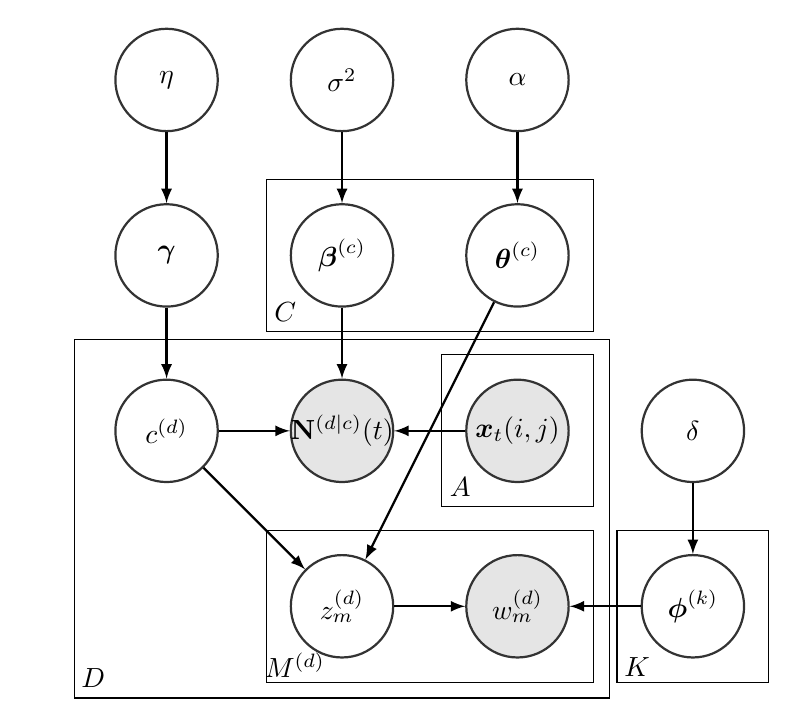
\begin{tikzpicture}
 	\tikzstyle{main}=[circle, minimum size = 13mm, thick, draw =black!80, node distance = 9mm]
 	\tikzstyle{connect}=[-latex, thick]
 	\tikzstyle{box}=[rectangle, draw=black!100]
 	\node[main, fill = white!100] (gamma) [label=center:$\boldsymbol{\gamma}$] { };
 	\node[main] (c) [below=of gamma,label=center:$c^{(d)}$] { };
 		\node[main, fill = black!10] (N) [right=of c ,label=center:$\mathbf{N}^{(d|c)}(t)$] { };	
 		\node[main] (z) [below=of N,label=center:$z_m^{(d)}$] {};
 	\node[main, fill = black!10] (w) [right=of z,label=center:$w_m^{(d)}$] { };
 	\node[main] (phi) [right=of w,label=center:$\boldsymbol{\phi}^{(k)}$] { };
 	\node[main] (delta) [above=of phi,label=center:$\delta$] { };
 	 			\node[main] (eta) [above=of gamma,label=center:${\eta}$] { };
\node[main, fill = black!10] (x) [right=of N,label=center:$\boldsymbol{x}_t{(i,j)}$] { };
 	 		 	 						\node[main] (beta) [above=of N ,label=center:$\boldsymbol{\beta}^{(c)}$] { };
 	 		 	 							\node[main] (theta) [above=of x,label=center:$\boldsymbol{\theta}^{(c)}$] { };
 	 		 	 										 	\node[main] (alpha) [above=of theta,label=center:$\alpha$] { };
 	 		 	 						 	 		\node[main] (sigma) [above=of beta,label=center:$\sigma^2$] { };
 	\path (gamma) edge [connect] (c)
 	(z) edge [connect] (w)
 	(theta) edge [connect] (z)
 	(alpha) edge [connect] (theta)
 	(phi) edge [connect] (w)
 	(delta) edge [connect] (phi)
 	(sigma) edge [connect] (beta)
 	(x) edge [connect] (N)
 	(beta) edge [connect] (N)
 	(c) edge [connect] (N)
 	(c) edge [connect] (z)
 		(eta) edge [connect] (gamma);
 			\node[rectangle, inner sep=3mm, fit=  (x),label=below left:$A$, xshift=5mm, yshift=5mm] {};
 			\node[rectangle, inner sep=3mm,draw=black!100, fit= (beta)(theta)] {};
 				\node[rectangle, inner sep=4mm, fit=  (beta)(theta) ,label= below left:$C$, xshift=-5mm, yshift=6mm] {};
 	\node[rectangle, inner sep=3mm, draw=black!100, fit= (phi)] {};
 		\node[rectangle, inner sep=3mm, draw=black!100, fit= (x) ] {};
 		\node[rectangle, inner sep=0mm, fit= (phi),label=below left:$K$, xshift=2.5mm, yshift=1.5mm] {};
 	\node[rectangle, inner sep=0mm, fit= (w),label=below left:$M^{(d)}$, xshift=-16.5mm, yshift=2mm] {};
 	\node[rectangle, inner sep=3mm,draw=black!100, fit= (w)(z)] {};
 	\node[rectangle, inner sep=3mm, fit= (c) (z) (w) (N) (x) ,label=below left:$D$, xshift=-8mm, yshift=3mm] {};
 	\node[rectangle, inner sep=5mm, draw=black!100, fit =(c) (z) (w) (N) (x) ] {};
 	\end{tikzpicture}}
 	\caption{Plate notation of IPTM}
 	\label{fig:plate}
 \end{figure}
 \begin{table}[ht]
 	 \centering
\scalebox{0.8}{ 	\begin{tabular}{ |c|c|c|} 
	\hline
 		\hline
 	Authors of the corpus &$\mathcal{A}$ & Set\\
 		\hline
 			Authors of the corpus given interaction pattern $c$ &$\mathcal{A}^{(c)}$ & Set\\
 			\hline
 	Number of authors &$A$ & Scalar \\
 		\hline
 		 	Number of documents &$D$ & Scalar \\
 		 	\hline
 		 	 	Number of words in the $d^{th}$ document &$M^{(d)}$ & Scalar \\
 		 	 	\hline
  	Number of topics & $K$ & Scalar \\
  	\hline
  	  Vocabulary size & $W$ & Scalar \\
  	  	\hline
  	 	Number of interaction patterns &$C$ & Scalar \\
  	 	\hline
  	 		Number of words assigned to interaction pattern and topic&$M^{CK}$ & Scalar \\
  	 		\hline
  	 			Number of words assigned to word and topic&$M^{WK}$ & Scalar \\
  	 			\hline
  	 	Interaction pattern of the $d^{th}$ document&$c^{(d)}$ & Scalar\\
  	 	\hline 
  	 	Time of the $d^{th}$ document&$t^{(d)}$ & Scalar\\
  	 		\hline 
  		Words in the $d^{th}$ document&$\boldsymbol{w}^{(d)}$ & $M^{(d)}$-dimensional vector\\
  		\hline 
  			$m^{th}$ word in the $d^{th}$ document&${w}_m^{(d)}$ & $m^{th}$  component of $\boldsymbol{w}^{(d)}$\\
  			\hline 	
  				Topic assignments in the $d^{th}$ document&$\boldsymbol{z}^{(d)}$ & $M^{(d)}$-dimensional vector\\
  				\hline 
  				Topic assignments for $m^{th}$ word in the $d^{th}$ document&${z}_m^{(d)}$ & $m^{th}$  component of $\boldsymbol{z}^{(d)}$\\
  				\hline 	
  				Dirichlet concentration prior&$\alpha$ & Scalar \\
  					\hline	
  				Dirichlet base prior&$\boldsymbol{m}$ & $K$-dimensional vector \\
  									\hline			
  							Dirichlet concentration prior&$\delta$ & Scalar \\
  							\hline			 
  								Dirichlet base prior&$\boldsymbol{n}$ & $W$-dimensional vector  \\
  								\hline				 	
  									Dirichlet concentration  prior&$\eta$ & Scalar \\
  									\hline		
  										Dirichlet base prior&$\boldsymbol{l}$ & $C$-dimensional vector  \\
  										\hline			
  				Multinomial prior&$\gamma$ & $C$-dimensional vector \\
  				\hline
  				Variance of Normal prior&$\sigma^2$ & Scalar \\
  				\hline		
  					Probabilities of the words given topics &$\Phi$ & $W \times K$ matrix \\
  					\hline		
  						Probabilities of the words given topic $k$ &$\boldsymbol{\phi}^{(k)}$ & $W$-dimensional vector\\
  						\hline
  							Probabilities of the topics given interaction patterns &$\Theta$ & $K \times C$ matrix \\
  							\hline		
  							Probabilities of the topics given interaction pattern $c$ &$\boldsymbol{\theta}^{(c)}$ & $K$-dimensional vector\\
  						\hline		
  						Coefficient of the intensity process given interaction pattern $c$ &$\boldsymbol{\beta}^{(c)}$ & $p$-dimensional vector\\
  							\hline		
  					Network statistics for directed edge $(i, j)$ &$\boldsymbol{x}_t{(i,j)}$ & $p$-dimensional vector\\
  						\hline		
  				Counting process in the $d^{th}$ document given interaction pattern &	$\mathbf{N}^{(d|c)}(t)$ & $A\times A$ matrix\\
  						\hline
  						\hline
 	\end{tabular}}
 	\caption {Symbols associated with IPTM, as used in this work}
 	\label{table:SymbolsIPTM}
 \end{table}
\normalsize
\subsection{Dynamic covariates to measure network effects}
The network statistics $\boldsymbol{x}_t(i, j)$ of equations (2), corresponding to the ordered pair $(i, j)$, can be time-invariant (such as gender) or time-dependent (such as the number of two-paths from $i$ to $j$ just before time $t$). Since time-invariant covariates can be easily specified in various manners (e. g. homophily or group-level effects), here we only consider specification of dynamic covariates.\\ \newline
Following \cite{PerryWolfe2012}, we use 6 effects as components of $\boldsymbol{x}_t(i, j)$. The first two behaviors (send and receive) are dyadic, involving exactly two actors,
while the last four (2-send, 2-receive, sibling, and cosibling) are triadic, involving exactly three actors.  In addition, we include intercept term and use $\boldsymbol{x}^*_t(i, j)$ so that we can estimate the baseline intensities at the same time. One different thing is that we define the effects not to be based on finite sub-interval, which require large number of dimention. Instead, we create a single statistic for each effect by incorporating the recency of event into the statistic itself. 
\begin{itemize}[leftmargin=*,rightmargin=-1cm ]
\item [0.] $\mbox{intercept}_t(i, j) = 1$
\item [1.]  $\mbox{send}_t(i, j)=\sum\limits_{d: t^{(d)}<t} I\{i\rightarrow j\}\cdot g(t-t^{(d)})$
\item [2.] $\mbox{receive}_t(i, j)=\sum\limits_{d: t^{(d)}<t} I\{j\rightarrow i\}\cdot g(t-t^{(d)})$
\item [3.] $\mbox{2-send}_t(i, j)=\sum\limits_{h \neq i, j}\Big(\sum\limits_{d: t^{(d)}<t}  I\{i\rightarrow h\}\cdot g(t-t^{(d)})\Big)\Big(\sum\limits_{d: t^{(d)}<t} I\{h\rightarrow j\}\cdot g(t-t^{(d)})\Big)$
\item [4.]  $\mbox{2-receive}_t(i, j)=\sum\limits_{h \neq i, j}\Big(\sum\limits_{d: t^{(d)}<t} I\{h\rightarrow i\}\cdot g(t-t^{(d)})\Big)\Big(\sum\limits_{d: t^{(d)}<t} I\{j\rightarrow h\}\cdot g(t-t^{(d)})\Big)$
\item [5.] $\mbox{sibling}_t(i, j)=\sum\limits_{h \neq i, j}\Big(\sum\limits_{d: t^{(d)}<t} I\{h\rightarrow i\}\cdot g(t-t^{(d)})\Big)\Big(\sum\limits_{d: t^{(d)}<t} I\{h\rightarrow j\}\cdot g(t-t^{(d)})\Big)$
\item [6.] $\mbox{cosibling}_t(i, j)=\sum\limits_{h \neq i, j}\Big(\sum\limits_{d: t^{(d)}<t} I\{i\rightarrow h\}\cdot g(t-t^{(d)})\Big)\Big(\sum\limits_{d: t^{(d)}<t} I\{j\rightarrow h\}\cdot g(t-t^{(d)})\Big)$
\end{itemize}
Here, $g(t-t^{(d)})$ reflects the difference between current time $t$ and the timestamp of previous email $t^{(d)}$, thus measuring the recency. Inspired by the self-exciting Hawkes process, which is often used to model the temporal effect of email data, we can take the exponential kernel $g(t-t^{(d)})=\lambda e^{-\lambda(t-t^{(d)})}$ where $\lambda$ is the parameter of speed at
which sender replies to emails, with larger values indicating faster response times. Indeed, $\lambda^{-1}$ is the expected number of hours it takes to reply to a typical email. For simplicity, we can fix $\lambda=1$.
\subsection{Inference}
The inference for IPTM is similar to that of CPME. In this case, what we actually observe are the  tokens $\mathcal{W}=\{\boldsymbol{w}^{(d)} \}_{d=1}^{D}$ and the counting process $\mathcal{N}=\{\boldsymbol{N}^{(d)}(\Delta t^{(d)}) \}_{d=1}^{D}.$ Next,  $\mathcal{X}=\{\boldsymbol{x}_{t^{(d)}}(i, j)\}_{d=1}^{D}$ is the metadata, and the latent variables are $\Phi=\{\boldsymbol{\phi}^{(k)}\}_{k=1}^{K}, \Theta=\{\boldsymbol{\theta}^{(c)} \}_{c=1}^{C}, \mathcal{Z}=\{\boldsymbol{z}^{(d)} \}_{d=1}^{D}, \mathcal{C}=\{{c}^{(d)} \}_{d=1}^{D},$ and $\mathcal{B}=\{\boldsymbol{\beta}^{(c)} \}_{c=1}^{C}$.\\
\newline 
Below is the the big joint distribution
\begin{equation}
\begin{aligned}
& P(\Phi, \Theta, \mathcal{W}, \mathcal{Z}, \mathcal{C}, \mathcal{B}, \mathcal{N}| \mathcal{X}, \delta, \boldsymbol{n}, \alpha, \boldsymbol{m}, \boldsymbol{\gamma}, \boldsymbol{\eta}, \sigma^2) \\& 
=  P(\mathcal{W}, \mathcal{Z}, \mathcal{C}, \mathcal{B}, \mathcal{N}| \Phi, \Theta, \mathcal{X}, \boldsymbol{\gamma}, \boldsymbol{\eta}, \sigma^2) P(\Phi, \Theta |\delta, \boldsymbol{n}, \alpha, \boldsymbol{m})
\\&= P( \mathcal{W}| \mathcal{Z}, \Phi)P(\mathcal{Z}|\Theta)P(\mathcal{N}|\mathcal{C}, \mathcal{X}, \mathcal{B})P(\mathcal{B}|\mathcal{C}, \sigma^2)P(\Phi|\delta, \boldsymbol{n})P(\Theta|\mathcal{C}, \alpha, \boldsymbol{m})P(\mathcal{C}|\boldsymbol{\gamma})P(\boldsymbol{\gamma}|\boldsymbol{\eta})
\end{aligned}
\end{equation}
Now we can integrate out $\Phi$ and $\Theta$ in latent Dirichlet allocation by applying Dirichlet-multinomial conjugacy as we did in CPME. See APPENDIX A for the detailed steps. After integration, we obtain below:
\begin{equation}
\propto P(\mathcal{W}|\mathcal{Z})P( \mathcal{Z}|\mathcal{C}, \delta, \boldsymbol{n}, \alpha, \boldsymbol{m})P(\mathcal{N}|\mathcal{C}, \mathcal{B}, \mathcal{X})P(\mathcal{B}|\mathcal{C}, \sigma^2)P(\mathcal{C}|\boldsymbol{\gamma})
\end{equation}
Then, we only have to perform inference over the remaining unobserved latent variables $\mathcal{Z}, \mathcal{C},$ and $\mathcal{B}$, using the equation below:
\begin{equation}
P( \mathcal{Z}, \mathcal{C}, \mathcal{B}|\mathcal{W}, \mathcal{N}, \mathcal{X}, \delta, \boldsymbol{n}, \alpha, \boldsymbol{m}, \boldsymbol{\gamma}, \boldsymbol{\eta}, \sigma^2) \propto P(\mathcal{W},  \mathcal{Z}, \mathcal{C}, \mathcal{B}, \mathcal{N} | \mathcal{X}, \delta, \boldsymbol{n}, \alpha, \boldsymbol{m}, \boldsymbol{\gamma}, \boldsymbol{\eta}, \sigma^2)
\end{equation}
 Either Gibbs sampling or Metropolis-Hastings algorithm is applied by sequentially resampling each latent variables from their respective conditional posterior.
  \subsubsection{Resampling $\mathcal{C}$}
  The first variable we are going to resample is the document-interaction pattern assignments, one document at a time. For this, we will use the Metropolis-Hastings algorithm with a proposal density $Q$ being the discrete uniform distribution over [1, $C$], which means that it does not depend on the
previous value of the chain. Then we draw a proposal $c$ at each iteration. Under symmetric proposal distribution (such as our case of discrete uniform), we cancel out Q-ratio and obtain the acceptance probability equal to:
\begin{equation}
\begin{split}
& \mbox{Acceptance Probability}=
\begin{cases}  \frac{P(\mathcal{C'}|\mathcal{W}, \mathcal{Z}, \mathcal{B}, \mathcal{N}, \mathcal{X}, \delta, \boldsymbol{n}, \alpha, \boldsymbol{m}, \boldsymbol{\gamma}, \boldsymbol{\eta}, \sigma^2)}{P(\mathcal{C}|\mathcal{W}, \mathcal{Z}, \mathcal{B}, \mathcal{N}, \mathcal{X}, \delta, \boldsymbol{n}, \alpha, \boldsymbol{m}, \boldsymbol{\gamma}, \boldsymbol{\eta}, \sigma^2)}\quad\text{if}  <1\\
1 \quad \text{else}
\end{cases}
\end{split}
\end{equation}
To obtain the acceptance probability, we need to obtain an expression for the conditional probability $P(c^{(d)}=c|\mathcal{W}, \mathcal{Z},  \mathcal{C}_{\backslash d}, \mathcal{B}, \mathcal{N}, \mathcal{X}, \delta, \boldsymbol{n}, \alpha, \boldsymbol{m}, \boldsymbol{\gamma}, \boldsymbol{\eta}, \sigma^2)$. 
  The conditional posterior probability we want to calculate is:
  \begin{equation}
  \begin{aligned} & P(c^{(d)}=c|\mathcal{W}, \mathcal{Z}, \mathcal{C}_{\backslash d}, \mathcal{B}, \mathcal{N}, \mathcal{X}, \delta, \boldsymbol{n}, \alpha, \boldsymbol{m}, \boldsymbol{\gamma}, \boldsymbol{\eta}, \sigma^2)\\
  &\propto P(c^{(d)}=c, \boldsymbol{w}^{(d)}, \boldsymbol{z}^{(d)},  \mathbf{N}{(\Delta t^{(d)})}|\mathcal{W}_{\backslash d}, \mathcal{Z}_{\backslash d},\mathcal{C}_{\backslash d}, \mathcal{B}, \mathcal{N}_{\backslash d}, \mathcal{X}, \delta, \boldsymbol{n}, \alpha, \boldsymbol{m}, \boldsymbol{\gamma}, \boldsymbol{\eta}, \sigma^2)\\& \propto P(c^{(d)}=c|\mathcal{C}_{\backslash d}, \boldsymbol{\gamma}) P( \mathbf{N}{(\Delta t^{(d)})}=n| c^{(d)}=c, \mathcal{C}_{\backslash d}, \mathcal{B}, \mathcal{N}_{\backslash d}, \mathcal{X})P(\boldsymbol{w}^{(d)}, \boldsymbol{z}^{(d)}|c^{(d)}=c, \mathcal{W}_{\backslash d}, \mathcal{Z}_{\backslash d}, \mathcal{C}_{\backslash d}, \delta, \boldsymbol{n}, \alpha, \boldsymbol{m}) 
 \end{aligned}
  \end{equation}
  Using Bayes' theorem (See APPENDIX B for conditional probabilty of the last term), we have
   \begin{equation}
   \begin{aligned} &=\Big[ \gamma_{c}\Big]\times\Big[\Big( \mbox{exp}\Big\{{-(t^{(d)}-t^{(d-1)})\sum\limits_{i \in \mathcal{A}^{(c)}}\sum\limits_{j\in \mathcal{A}^{(c)}}\lambda_{ij}^{(c)}(t^{(d)})}\Big\}\cdot \prod_{i \in \mathcal{A}^{(c)}}\prod_{j\in \mathcal{A}^{(c)}}\frac{\Big(\lambda_{ij}^{(c)}(t^{(d)})\cdot(t^{(d)}-t^{(d-1)})\Big)^{n_d^{(ij)}}}{n_d^{(ij)}!}\Big)\Big]\\&\quad\times\Big[\prod_{m=1}^{M^{(d)}}
    \frac{M^{CK}_{cz_m^{(d)}, \backslash d, m}+\alpha m_k}{\sum_{k=1}^KM^{CK}_{ck, \backslash d, m}+\alpha}\Big]
   \end{aligned}
   \end{equation}
where $M^{CK}_{ck}$ is the number of times topic k shows up given the interaction pattern $c$ and $\lambda_{ij}^{(c)}(t^{(d)})=\mbox{exp}\Big\{\boldsymbol{\beta}^{(c)T}\boldsymbol{x}^*_{t^{(d)}}(i, j)\Big\}\cdot 1\{j \in \mathcal{A}^{(c)}\}$. Moreover, since our $n_d^{(ij)}$ is either 0 or 1, Equation (10) can be simplified as below:
  	\begin{equation} \gamma_{c}\cdot \mbox{exp}\Big\{{-(t^{(d)}-t^{(d-1)})\big(\sum\limits_{i \in  \mathcal{A}^{(c)}}\sum\limits_{j\in \mathcal{A}^{(c)}}\lambda_{ij}^{(c)}(t^{(d)})\big)}\Big\}\cdot \lambda_{i^{(d)}j^{(d)}}^{(c)}(t^{(d)})(t^{(d)}-t^{(d-1)})\cdot \Big[\prod_{m=1}^{M^{(d)}}
  	\frac{M^{CK}_{cz_m^{(d)}, \backslash d, m}+\alpha m_k}{\sum_{k=1}^KM^{CK}_{ck, \backslash d, m}+\alpha}\Big]
  	\end{equation}
  	Furthermore, we can speed up the computation time by taking the log of Equation (11), which becomes:
  	 \begin{equation}
\mbox{log}(\gamma_{c})-(t^{(d)}-t^{(d-1)})\big(\sum\limits_{i \in \mathcal{A}^{(c)}}\sum\limits_{j\in \mathcal{A}^{(c)}}\lambda_{ij}^{(c)}(t^{(d)})\big)+\mbox{log}\Big(\lambda_{i^{(d)}j^{(d)}}^{(c)}(t^{(d)})(t^{(d)}-t^{(d-1)})\Big)+\sum_{m=1}^{M^{(d)}}\mbox{log}(\frac{M^{CK}_{cz_m^{(d)}, \backslash d, m}+\alpha m_k}{\sum_{k=1}^KM^{CK}_{ck, \backslash d, m}+\alpha})
  	 \end{equation}
  	 Then, by applying the above to Equation (8) and replacing $\lambda_{ij}^{(c)}(t^{(d)})$ to $\mbox{exp}\Big\{\boldsymbol{\beta}^{(c)T}\boldsymbol{x}^*_{t^{(d)}}(i, j)\Big\}, $, the log of the acceptance ratio we have is:
  	   	 \begin{equation}
  	   	 \begin{aligned} &\mbox{log}(\gamma_{c^\prime})-\mbox{log}(\gamma_{c}) +\Big(\boldsymbol{\beta}^{(c')T}-\boldsymbol{\beta}^{(c)T}\Big)\boldsymbol{x}^*_{t^{(d)}}(i^{(d)}, j^{(d)})\\& \quad-(t^{(d)}-t^{(d-1)})\sum\limits_{i \in A^{(c)}}\sum\limits_{j\in \mathcal{A}^{(c)}}\Big(\mbox{exp}\Big\{\boldsymbol{\beta}^{(c')T}\boldsymbol{x}^*_{t^{(d)}}(i, j)\Big\}-\mbox{exp}\Big\{\boldsymbol{\beta}^{(c)T}\boldsymbol{x}^*_{t^{(d)}}(i, j)\Big\}\Big)\\&\quad+\sum_{m=1}^{M^{(d)}}\Big(\mbox{log}({M^{C'K}_{c'z_m^{(d)}, \backslash d, m}+\alpha m_k})-\mbox{log}({\sum_{k=1}^KM^{C'K}_{c'k, \backslash d, m}+\alpha})-\mbox{log}({M^{CK}_{cz_m^{(d)}, \backslash d, m}+\alpha m_k})+\mbox{log}({\sum_{k=1}^KM^{CK}_{ck, \backslash d, m}+\alpha})\Big)
  	 \end{aligned}
  	 \end{equation}
 Following the typical Metropolis-Hastings approach, we use the log of the acceptance ratio:
  	 \begin{equation}
  	 \mbox{log(Acceptance Probability) = min((13), 0) }
  	 \end{equation}
  	 To determine whether we accept the proposed update or not, we take the usual approach, by comparing the log of acceptance ratio we have to the log of a sample from uniform(0,1).
\subsubsection{Resampling $\mathcal{Z}$}
Next, the new values of $z^{(d)}_m$ are sampled for all of the token topic assignments (one token at a time), using the conditional posterior probability of being topic $k$ as we derived in APPENDIX B:
\begin{equation}
\begin{aligned} & 
 P(z^{(d)}_m=k|\mathcal{W}, \mathcal{Z}_{\backslash d, m},  \mathcal{C}, \mathcal{B}, \mathcal{N}, \mathcal{X}, \delta, \boldsymbol{n}, \alpha, \boldsymbol{m}, \boldsymbol{\gamma}, \boldsymbol{\eta}, \sigma^2)\\
& \propto P(z^{(d)}_m=k, w^{(d)}_m|\mathcal{W}_{\backslash d, m}, \mathcal{Z}_{\backslash d,m}, C, \delta, \boldsymbol{n}, \alpha, \boldsymbol{m})
\end{aligned}
\end{equation}
where the subscript $``{\backslash d, m}"$ denotes the exclsuion of position $m$ in email $d$. In the last line of equation (10), it is the contribution of LDA, so similar to CPME we can write the conditional probability:
	\begin{equation}
	\begin{aligned} 
	& \propto(M^{CK}_{c^{(d)}k, \backslash d, m}+\alpha m_k)\cdot\frac{M_{w_m^{(d)}k, \backslash d, m}^{WK}+\delta n_w}{\sum_{w=1}^WM_{wk,  \backslash d, m}^{WK}+\delta}
	\end{aligned}
	\end{equation}
	which is the well-known form of collapsed Gibbs sampling equation for LDA.
\subsubsection{Resampling $\mathcal{B}$}
Finally, we wan to update the interaction pattern parameter $\boldsymbol{\beta}^{(c)}$, one interaction pattern at a time. For this, we will use the Metropolis-Hastings algorithm with a proposal density $Q$ being the multivariate Gaussian distribution, with variance $\sigma^2$, centered on the current values of $\boldsymbol{\beta}^{(c)}$. Then we draw a proposal $\boldsymbol{\beta}'^{(c)}$ at each iteration. Under symmetric proposal distribution (such as multivariate Gaussian), we cancel out Q-ratio and obtain the acceptance probability equal to:
\begin{equation}
\begin{split}
& \mbox{Acceptance Probability}=
\begin{cases}  \frac{P(\mathcal{B'}|\mathcal{W}, \mathcal{Z}, \mathcal{C}, \mathcal{N}, \mathcal{X})}{P(\mathcal{B}|\mathcal{W}, \mathcal{Z}, \mathcal{C}, \mathcal{N}, \mathcal{X})}\quad\text{if}  <1\\
1 \quad \text{else}
\end{cases}
\end{split}
\end{equation}
After factorization, we get
\begin{equation}
\begin{aligned}
\frac{P(\mathcal{B'}|\mathcal{W},\mathcal{Z}, \mathcal{C}, \mathcal{N}, \mathcal{X})}{P(\mathcal{B}|\mathcal{W}, \mathcal{Z}, \mathcal{C}, \mathcal{N}, \mathcal{X})} &=\frac{P(\mathcal{N}|\mathcal{B'}, \mathcal{W}, \mathcal{Z}, \mathcal{C}, \mathcal{X})P(\mathcal{B'})}{P(\mathcal{N}|\mathcal{B}, \mathcal{W}, \mathcal{Z},  \mathcal{C}, \mathcal{X})P(\mathcal{B})}\\&=\frac{P(\mathcal{N}|\mathcal{C}, \mathcal{X}, \mathcal{B'})P(\mathcal{B'})}{P(\mathcal{N}|\mathcal{C}, \mathcal{X}, \mathcal{B})P(\mathcal{B})}.
\end{aligned}
\end{equation}
Since $P(\mathcal{N}|\mathcal{C}, \mathcal{X}, \mathcal{B})$ represents the multivariate counting process contribution in \cite{zocher2006multivariate} we already used in Equation (8). The full probability of observing the edges under the interaction pattern parameters is: \begin{equation}
\prod_{d:c^{(d)}=c}\Big(\mbox{exp}\Big\{{-(t^{(d)}-t^{(d-1)})\sum\limits_{i \in \mathcal{A}^{(c)}}\sum\limits_{j\in \mathcal{A}^{(c)}}\lambda_{ij}^{(c)}(t^{(d)})}\Big\}\cdot \prod_{i \in \mathcal{A}^{(c)}}\prod_{j\in \mathcal{A}^{(c)}}\frac{\Big(\lambda_{ij}^{(c)}(t^{(d)})\cdot(t^{(d)}-t^{(d-1)})\Big)^{n_d^{(ij)}}}{n_d^{(ij)}!}\Big).
\end{equation}
For $P(\mathcal{B})$, we select a multivarate Gaussian priors as mentioned earlier. Similar to what we did in Section 2.4.1, we can use the simplified equation as in Equation (11) and take the log, then we obtain the log of acceptance ratio as following:
\begin{equation}
\begin{aligned} 
&\mbox{log}(P(\mathcal{B'}))-\mbox{log}(P(\mathcal{B}))+\sum_{d:c^{(d)}=c}\Big(\boldsymbol{\beta'}^{(c)T}-\boldsymbol{\beta}^{(c)T}\Big)\boldsymbol{x}^*_{t^{(d)}}(i^{(d)}, j^{(d)})\\&-\sum_{d:c^{(d)}=c}\Big((t^{(d)}-t^{(d-1)})\sum\limits_{i \in A^{(c)}}\sum\limits_{j\in \mathcal{A}^{(c)}}\Big(\mbox{exp}\Big\{\boldsymbol{\beta'}^{(c)T}\boldsymbol{x}^*_{t^{(d)}}(i, j)\Big\}-\mbox{exp}\Big\{\boldsymbol{\beta}^{(c)T}\boldsymbol{x}^*_{t^{(d)}}(i, j)\Big\}\Big)\Big)
\end{aligned}
\end{equation}
Then the log of acceptance ratio we have is:
\begin{equation}
\mbox{log(Acceptance Probability) = min((20), 0) }
\end{equation}
To determine whether we accept the proposed update or not, we take the usual approach, by comparing the log of acceptance ratio we have to the log of a sample from uniform(0,1).
\begin{comment}
\section{Preliminary Analysis}
Hurricane Sandy was the most destructive hurricane in 2012, which hit North Carolina on late October (October 28, Governor Bev Perdue declared a state of emergency in 24 western counties due to snow and strong winds). In our dataset, there are three counties which cover the date of Hurricane Sandy (October 22, 2012 – November 2, 2012), so we focus on the three counties, since the timestamp of email in this case is much more important than usual case without any disastrous event.
\subsection{Dare County}
\footnotesize
\begin{table}[ht]
	\centering
	\begin{tabular}{ |c|ccc|c| } 
		\hline 
		\textbf{Period} &\textbf{Before Sandy} & \textbf{During Sandy} & \textbf{After Sandy} & \textbf{Overall} \\ 	\hline
			\textbf{\# emails}& 1933 & 1563 & 1467 & 4963 \\ 
		\hline
	\end{tabular}
	\caption{ Summary of Dare county email data based on time period}
	\label{table:nullDare2}
\end{table}
\normalsize
Before Sandy ranges from 2012-09-01 to 2012-10-21 (7 weeks), During Sandy ranges from 2012-10-22 to 2012-11-02 (2 weeks), and After Sandy ranges from 2012-11-03 to 2012-11-30 (4 weeks).
\footnotesize
\begin{figure}[ht]
	\centering
	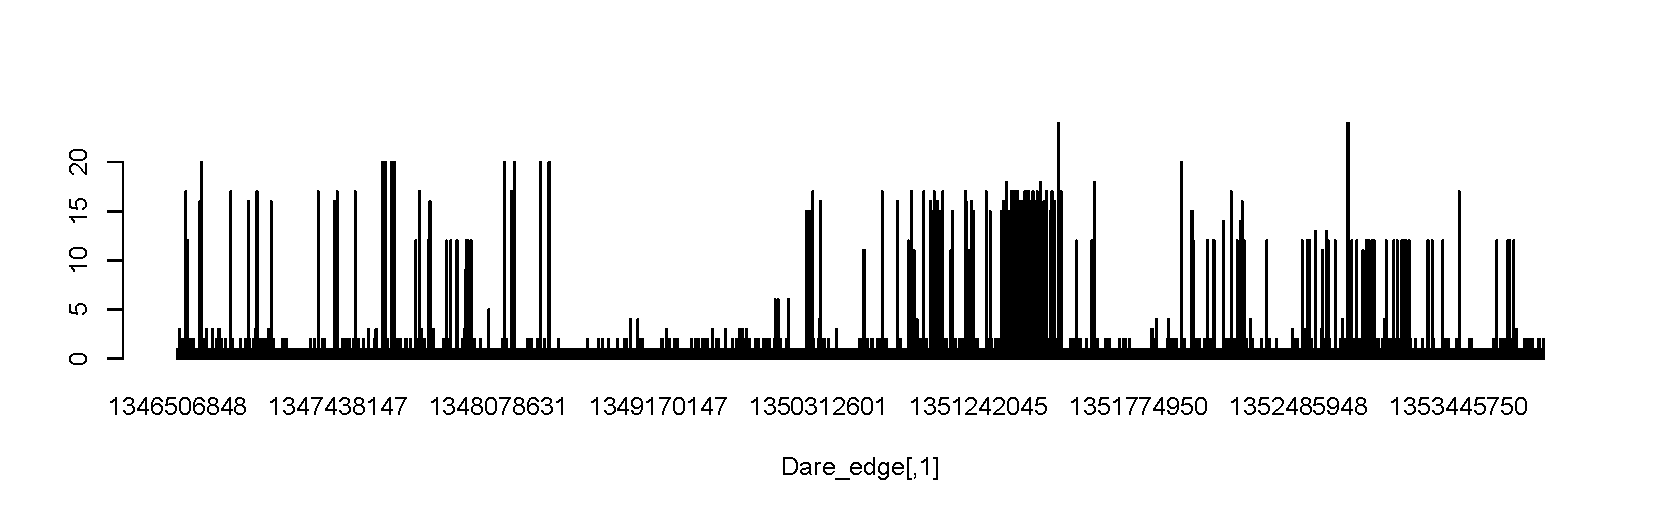
\includegraphics[width=1.1\textwidth]{DareEmails.pdf} 
	\caption{Frequency of Dare county emails from 2012-09-01 to 2012-11-30  }
	\label{fig:Emailplots}
\end{figure}
\begin{table}[ht]
	\centering
	\begin{tabular}{ |c|cc| } 
		\hline 
		\textbf{Time Interval} &\textbf{send} & \textbf{receive} \\ 	
		\hline  $[-\infty, t)$&  2.128, 2.659, 2.355, 2.919& 0.292, 0.257, 0.047, 0.110\\  $[t-30 m, t)$ &  0.262, -0.064, 0.782, 0.317 &2.087, 1.287 , 2.346, 1.870\\  $[t-2h, t-30m)$& 0.383, 0.157 , 0.024, -0.045 &0.553, 0.082, 0.794, 0.269\\ $[t-8h, t-2h)$ & 0.816, 0.054 , 0.077, 0.381 &-0.221, 0.048, 0.298, -0.012 \\ $[t-32h, t-8h)$& 0.085, 0.014,  0.228, 0.070 &0.101, 0.017, -0.033, 0.019\\ $[t-5.33d, t-32h)$&  0.103, 0.025, 0.092, 0.008 &-0.027, -0.016, -0.033, -0.009 \\ $[t-21.33d, t-5.33d)$  & 0.052, 0.000, 0.059, 0.010& 0.013, 0.030 , -0.016, 0.013\\ 
		$[-\infty, t-21.33d)$  & 0.052, 0.103, 0.027, 0.021  & 0.008, 0.000, 0.020, -0.005\\
		\hline
	\end{tabular}
	\caption {Estimated coefficients and approximate standard errors for dyadic effects of Dare county data (before Sandy, during Sandy, after Sandy, overall)}
	\label{table:nullDare}
\end{table}
\footnotesize
\begin{figure}[ht]
	\centering
	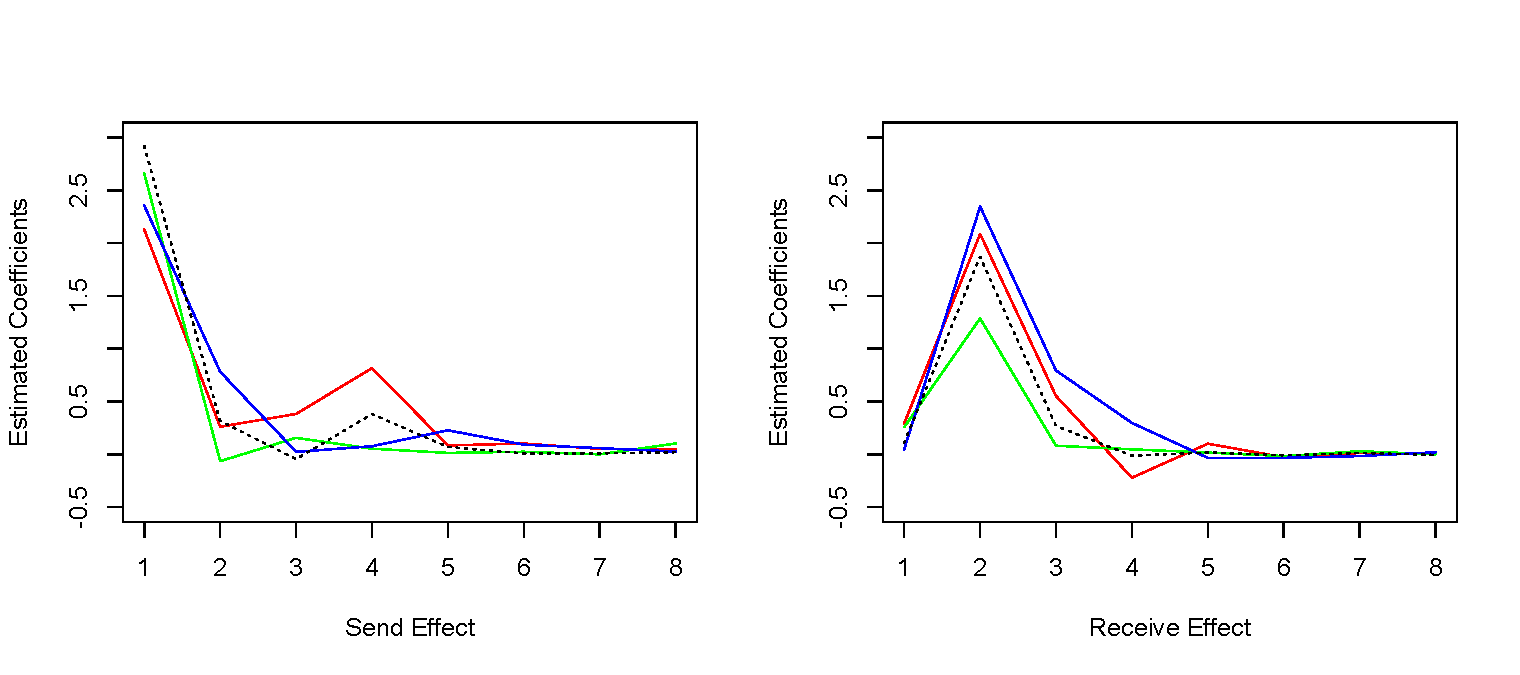
\includegraphics[width=1.1\textwidth]{Dareplot.pdf} 
	\caption{Comparison of Send (left) and Receive (right) effect based on periods in Table 1. (Red=Before, Green=During, Blue=After, and dot=Overall)}	\label{fig:Emailplo22t}
\end{figure}
\subsection{Lenoir County}
\footnotesize
\begin{table}[ht]
	\centering
	\begin{tabular}{ |c|ccc|c| } 
		\hline 
		\textbf{Period} &\textbf{Before Sandy} & \textbf{During Sandy} & \textbf{After Sandy} & \textbf{Overall} \\ 	\hline
		\textbf{\# emails}& 216 & 83 & 302 & 601 \\ 
		\hline
	\end{tabular}
	\caption{ Summary of Lenoir county email data based on time period}
	\label{table:nullDare22}
\end{table}
\normalsize
Before Sandy ranges from 2012-10-01 to 2012-10-21 (3 weeks), During Sandy ranges from 2012-10-22 to 2012-11-02 (2 weeks), and After Sandy ranges from 2012-11-03 to 2012-12-31 (8 weeks).
\footnotesize
\begin{figure}[ht]
	\centering
	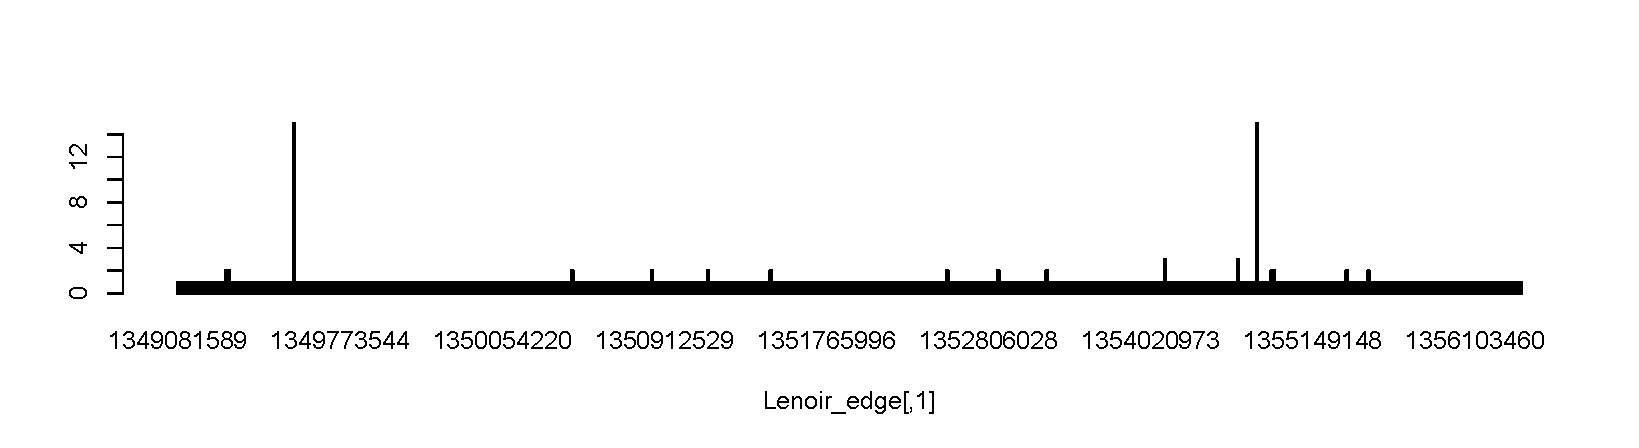
\includegraphics[width=1.1\textwidth]{LenoirEmails.pdf} 
	\caption{Frequency of Lenoir county emails from 2012-10-01 to 2012-12-31  }
	\label{fig:Emailplots32}
\end{figure}
\newpage
\subsection{Vance County}
\footnotesize
\footnotesize
\begin{table}[ht]
	\centering
	\begin{tabular}{ |c|ccc|c| } 
		\hline 
		\textbf{Period} &\textbf{Before Sandy} & \textbf{During Sandy} & \textbf{After Sandy} & \textbf{Overall} \\ 	\hline
		\textbf{\# emails}& 198& 18 & 55 & 271 \\ 
		\hline
	\end{tabular}
	\caption{ Summary of Vance county email data based on time period}
	\label{table:nullVance}
\end{table}
\normalsize
Before Sandy ranges from 2012-09-04 to 2012-10-21 (7 weeks), During Sandy ranges from 2012-10-22 to 2012-11-02 (2 weeks), and After Sandy ranges from 2012-11-03 to 2012-11-30  (4 weeks).
\footnotesize
\begin{figure}[ht]
	\centering
	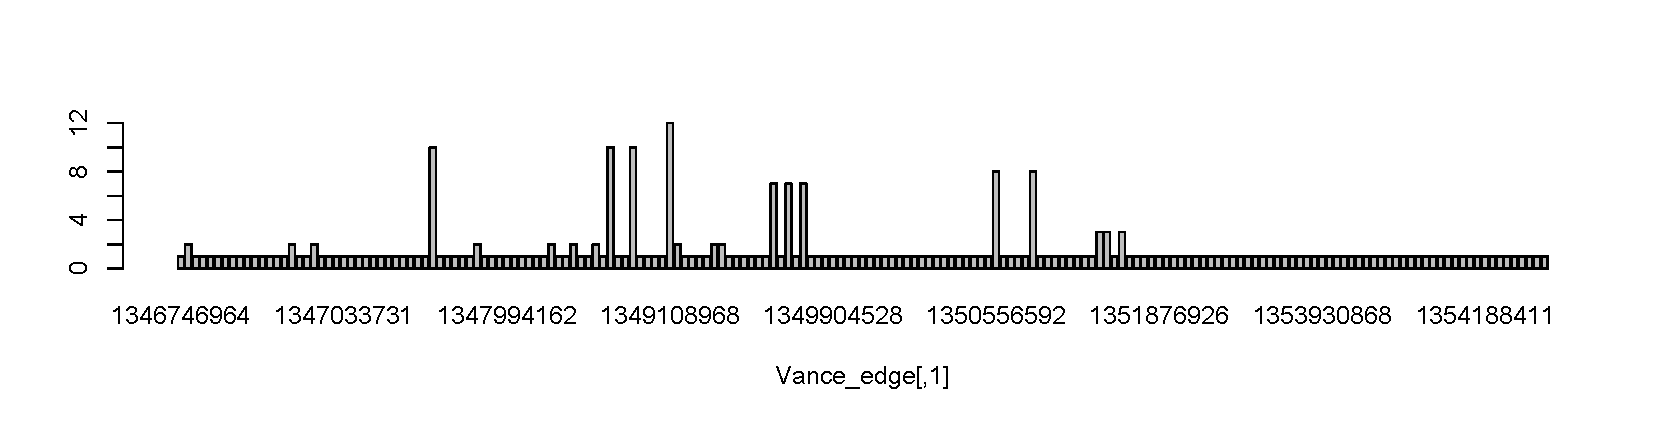
\includegraphics[width=1.1\textwidth]{VanceEmails.pdf} 
	\caption{Frequency of Vance county emails from 2012-09-04 to 2012-11-30  }
	\label{fig:Emailplots22}
\end{figure}
\end{comment}
\section*{APPENDIX}
\subsection*{APPENDIX A: Deriving the sampling equations for IPTM}
\begin{equation}
\begin{aligned}
& P(\Phi, \Theta, \mathcal{W}, \mathcal{Z}, \mathcal{C}, \mathcal{B}, \mathcal{N}| \mathcal{X}, \delta, \boldsymbol{n}, \alpha, \boldsymbol{m}, \boldsymbol{\gamma}, \boldsymbol{\eta}, \sigma^2) \\& 
=  P(\mathcal{W}, \mathcal{Z}, \mathcal{C}, \mathcal{B}, \mathcal{N}| \Phi, \Theta, \mathcal{X}, \boldsymbol{\gamma}, \boldsymbol{\eta}, \sigma^2) P(\Phi, \Theta |\delta, \boldsymbol{n}, \alpha, \boldsymbol{m})
\\&= P( \mathcal{W}| \mathcal{Z}, \Phi)P(\mathcal{Z}|\Theta)P(\mathcal{N}|\mathcal{C}, \mathcal{B}, \mathcal{X})P(\mathcal{B}|\mathcal{C}, \sigma^2)P(\Phi|\delta, \boldsymbol{n})P(\Theta|\mathcal{C}, \alpha, \boldsymbol{m})P(\mathcal{C}|\boldsymbol{\gamma})P(\boldsymbol{\gamma}|\boldsymbol{\eta})
\\&= \Big[\prod_{d=1}^{D}\prod_{m=1}^{M^{(d)}} P( w_m^{(d)}| \phi_{z_m^{(d)}})\Big]\times \Big[\prod_{d=1}^{D}\prod_{m=1}^{M^{(d)}} P( z_m^{(d)}| \boldsymbol{\theta}^{(c)})\Big]\times \Big[\prod_{d=1}^{D} P( \mathbf{N}^{(d)}(\Delta t^{(d)})| c^{(d)}, \boldsymbol{x}(t^{(d)}), \boldsymbol{\beta}^{(c)})\Big]  \\&\quad \quad \times\Big[\prod_{c=1}^{C} P( \boldsymbol{\beta}^{(c)}| \sigma^2)\Big]\times\Big[\prod_{k=1}^{K} P( \boldsymbol{\phi}^{(k)}| \delta, \boldsymbol{n})\Big]\times \Big[\prod_{c=1}^{C} P( \boldsymbol{\theta}^{(c)}|\alpha, \boldsymbol{m})\Big]\times \Big[\prod_{d=1}^{D} P(c^{(d)}|\boldsymbol{\gamma})\Big]  \times P(\boldsymbol{\gamma}|\boldsymbol{\eta})
\end{aligned}
\end{equation}
Since $P( \boldsymbol{\beta}^{(c)}| \sigma^2)$ is $\mbox{Normal}(\boldsymbol{0}, \sigma^2)$ and $P(\boldsymbol{\gamma}|\boldsymbol{\eta})$ is $\mbox{Dirichlet}(\boldsymbol{\eta})$, we can drop the two terms out and further rewrite the equation (20) as below:
\begin{equation}
\begin{aligned}
& \propto \Big[\prod_{d=1}^{D}\prod_{m=1}^{M^{(d)}} P( w_m^{(d)}| \phi_{z_m^{(d)}})\Big]\times \Big[\prod_{d=1}^{D}\prod_{m=1}^{M^{(d)}} P( z_m^{(d)}| \boldsymbol{\theta}^{(c)})\Big]\times \Big[\prod_{d=1}^{D} P( \mathbf{N}^{(d)}(\Delta t^{(d)})| c^{(d)}, \boldsymbol{x}(t^{(d)}), \boldsymbol{\beta}^{(c)})\Big]\\& \quad \quad  \times\Big[\prod_{k=1}^{K} P( \boldsymbol{\phi}^{(k)}| \delta, \boldsymbol{n})\Big] \times\Big[\prod_{c=1}^{C} P( \boldsymbol{\theta}^{(c)}|\alpha, \boldsymbol{m})\Big] \times\Big[\prod_{d=1}^{D} P(c^{(d)}|\boldsymbol{\gamma})\Big] \\&
= \Big[\prod_{d=1}^{D}\prod_{m=1}^{M^{(d)}} \phi_{w_m^{(d)}z_m^{(d)}}\Big]\times \Big[\prod_{d=1}^{D}\prod_{m=1}^{M^{(d)}} \boldsymbol{\theta}^{(c)}_{z_m^{(d)}}\Big]\\&\quad\quad\times\Big[\prod_{d=1}^{D} \Big(\mbox{exp}\Big\{{-(t^{(d)}-t^{(d-1)})\big(\sum\limits_{i \in \mathcal{A}^{(c^{(d)})}}\sum\limits_{j\in \mathcal{A}^{(c^{(d)})}}\lambda_{ij}^{(c^{(d)})}(t^{(d)})\big)}\Big\}\prod_{i \in  \mathcal{A}^{(c^{(d)})}}\prod_{j\in \mathcal{A}^{(c^{(d)})}}\frac{(\lambda_{ij}^{(c^{(d)})}(t^{(d)})(t^{(d)}-t^{(d-1)}))^{n_d^{(ij)}}}{n_d^{(ij)}!}\Big)\Big]\\& \quad \quad \times \Big[\prod_{k=1}^{K} \Big(\frac{\Gamma(\sum_{w=1}^{W}\delta n_w)}{\prod_{w=1}^{W}\Gamma(\delta n_w)}\prod_{w=1}^{W}\phi_{wk}^{\delta n_w-1} \Big)\Big]\times \Big[\prod_{c=1}^{C} \Big(\frac{\Gamma(\sum_{k=1}^{K}\alpha m_k)}{\prod_{k=1}^{K}\Gamma(\alpha m_k)}\prod_{k=1}^{K}(\boldsymbol{\theta}^{(c)}_{k})^{\alpha m_k-1} \Big)\Big] \times\Big[\prod_{d=1}^{D} \gamma_{c}^{I(c^{(d)}=c)}\Big] \\&
=\Big[\frac{\Gamma(\sum_{w=1}^{W}\delta n_w)}{\prod_{w=1}^{W}\Gamma(\delta n_w)}\Big]^K \\&\quad \quad \times \Big[\frac{\Gamma(\sum_{w=1}^{W}\delta n_w)}{\prod_{w=1}^{W}\Gamma(\delta n_w)}\Big]^C \times\Big[\prod_{d=1}^{D} \Big(\mbox{exp}\Big\{{-(t^{(d)}-t^{(d-1)})\big(\sum\limits_{i \in \mathcal{A}^{(c^{(d)})}}\sum\limits_{j\in \mathcal{A}^{(c^{(d)})}}\lambda_{ij}^{(c^{(d)})}(t^{(d)})\big)}\Big\}\cdot\lambda_{i^{(d)}j^{(d)}}^{(c^{(d)})}(t^{(d)})(t^{(d)}-t^{(d-1)})\Big)\Big]\\&\quad\quad\times\Big[\prod_{d=1}^{D}\gamma_{c^{(d)}}\Big]\times
\Big[\prod_{k=1}^{K}\prod_{w=1}^{W}\phi_{wk}^{M^{WK}_{wk}+\delta n_w-1}\Big]\times\Big[\prod_{c=1}^{C}\prod_{k=1}^{K}(\boldsymbol{\theta}^{(c)}_{k})^{M^{CK}_{ck}+\alpha m_k-1}\Big]
\end{aligned}
\end{equation}
where $M^{WK}_{wk}$ is the number of times the $w^{th}$ word in the vocabulary is assigned to topic $k$, and $M^{CK}_{ck}$ is the number of times topic k shows up given the interaction pattern $c$. By looking at the forms of the terms involving  $\Theta$ and $\Phi$ in Equation (21), we integrate out the random variables $\Theta$ and $\Phi$, making use of the fact that the Dirichlet distribution is a conjugate prior of multinomial distribution. Applying the well-known formula $\int\prod_{m=1}^{M}[x_m^{k_m-1}dx_m]=\frac{\prod_{m=1}^M\Gamma(k_m)}{\Gamma(\sum_{m=1}^Mk_m)}$ to (22), we have:
\begin{equation}
\begin{aligned}
&P(\mathcal{W}, \mathcal{Z}, \mathcal{C}, \mathcal{B}, \mathcal{N}| \mathcal{X}, \delta, \boldsymbol{n}, \alpha, \boldsymbol{m}, \boldsymbol{\gamma}, \boldsymbol{\eta}, \sigma^2)\\&=\mbox{Const.}\int_{\Theta}\int_{\Phi}\Big[\prod_{k=1}^{K}\prod_{w=1}^{W}\phi_{wk}^{M^{WK}_{wk}+\delta n_w-1}\Big]\Big[\prod_{c=1}^{C}\prod_{k=1}^{K}(\boldsymbol{\theta}^{(c)}_{k})^{M^{CK}_{ck}+\alpha m_k-1}\Big]d\Phi d\Theta
\\&=\mbox{Const.}\Big[\prod_{k=1}^{K}\int_{\phi_{:k}}\prod_{w=1}^{W}\phi_{wk}^{M^{WK}_{wk}+\delta n_w-1  }d\phi_{:k}\Big]\times\Big[\prod_{c=1}^{C}\int_{\theta_{:c}}\prod_{k=1}^{K}(\boldsymbol{\theta}^{(c)}_{k})^{M^{CK}_{ck}+\alpha m_k-1}d\theta_{:c}\Big]
\\&=\mbox{Const.}\Big[\prod_{k=1}^{K}\frac{\prod_{w=1}^W\Gamma(M_{wk}^{WK}+\delta n_w)}{\Gamma(\sum_{w=1}^WM_{wk}^{WK}+\delta )}\Big]\times\Big[\prod_{c=1}^{C}\frac{\prod_{k=1}^K\Gamma(M^{CK}_{ck}+\alpha m_k)}{\Gamma(\sum_{k=1}^KM^{CK}_{ck}+\alpha)}\Big].
\end{aligned}
\end{equation}
\subsection*{APPENDIX B: Computing conditional probability}
\begin{equation}
\begin{aligned}
& P(\boldsymbol{w}^{(d)}, \boldsymbol{z}^{(d)}|c^{(d)}=c, \mathcal{W}_{\backslash d}, \mathcal{Z}_{\backslash d}, \mathcal{C}_{\backslash d}, \delta, \boldsymbol{n}, \alpha, \boldsymbol{m}) \\& \propto \prod_{m=1}^{M^{(d)}}P(z^{(d)}_m=k, w^{(d)}_m=w| c^{(d)}=c, \mathcal{W}_{\backslash d, m}, \mathcal{Z}_{\backslash d,m}, \mathcal{C}_{\backslash d}, \delta, \boldsymbol{n}, \alpha, \boldsymbol{m})
\end{aligned}
\end{equation} 
To obtain the Gibbs sampling equation, we need to obtain an expression for $P(z^{(d)}_m=k,  w^{(d)}_m=w, c^{(d)}=c|\mathcal{W}_{\backslash d}, \mathcal{Z}_{\backslash d}, \mathcal{C}_{\backslash d}, \delta, \boldsymbol{n}, \alpha, \boldsymbol{m})$,
 From Bayes' theorem and Gamma identity $\Gamma(k+1)=k\Gamma(k)$,
\begin{equation}
\begin{aligned}
& P(z^{(d)}_m=k, w^{(d)}_m=w, c^{(d)}=c|\mathcal{W}_{\backslash d, m}, \mathcal{Z}_{\backslash d,m}, \mathcal{C}_{\backslash d}, \delta, \boldsymbol{n}, \alpha, \boldsymbol{m}) \\& \propto 
\frac{P(\mathcal{W}, \mathcal{Z}, \mathcal{C}|\delta, \boldsymbol{n}, \alpha, \boldsymbol{m})}{P(\mathcal{W}_{\backslash d, m}, \mathcal{Z}_{\backslash d, m}, \mathcal{C}|\delta, \boldsymbol{n}, \alpha, \boldsymbol{m})}\\& \propto \frac{\prod_{k=1}^{K}\frac{\prod_{w=1}^W\Gamma(M_{wk}^{WK}+\delta n_w)}{\Gamma(\sum_{w=1}^WM_{wk}^{WK}+\delta )}\times\prod_{c=1}^{C}\frac{\prod_{k=1}^K\Gamma(M^{CK}_{ck}+\alpha m_k)}{\Gamma(\sum_{k=1}^KM^{CK}_{ck}+\alpha)}}{\prod_{k=1}^{K}\frac{\prod_{w=1}^W\Gamma(M_{wk, \backslash d, m}^{WK}+\delta n_w)}{\Gamma(\sum_{w=1}^WM_{wk, \backslash d, m}^{WK}+\delta )}\times\prod_{c=1}^{C}\frac{\prod_{k=1}^K\Gamma(M^{CK}_{ck, \backslash d, m}+\alpha m_k)}{\Gamma(\sum_{k=1}^KM^{CK}_{ck, \backslash d, m}+\alpha)}}\\ & \propto 
\frac{M_{wk, \backslash d, m}^{WK}+\delta n_w}{\sum_{w=1}^WM_{wk,  \backslash d, m}^{WK}+\delta}\times\frac{M^{CK}_{ck, \backslash d, m}+\alpha m_k}{\sum_{k=1}^KM^{CK}_{ck, \backslash d, m}+\alpha}
\end{aligned}
\end{equation}
Then, the conditional probability that a novel word generated in the document of interaction pattern $c^{(d)}=c$  would be assigned to topic $z_m^{(d)}=k$ is obtained by:
 \begin{equation}
 \begin{aligned}
 &P(z^{(d)}_m=k|w^{(d)}_m=w, c^{(d)}=c, \mathcal{W}_{\backslash d, m}, \mathcal{Z}_{\backslash d,m}, \mathcal{C}_{\backslash d}, \delta, \boldsymbol{n}, \alpha, \boldsymbol{m}) \\& \propto
 \frac{M^{CK}_{ck, \backslash d, m}+\alpha m_k}{\sum_{k=1}^KM^{CK}_{ck, \backslash d, m}+\alpha}
 \end{aligned}
 \end{equation}
In addition, the conditional probability that a new word generated in the document would be $w_m^{(d)}=w$, given that it is generated from topic $z_m^{(d)}=k$ is obtained by:
\begin{equation}
\begin{aligned}
& P(w^{(d)}_m=w|z^{(d)}_m=k, c^{(d)}=c, \mathcal{W}_{\backslash d, m}, \mathcal{Z}_{\backslash d,m}, \mathcal{C}_{\backslash d}, \delta, \boldsymbol{n}, \alpha, \boldsymbol{m}) \\& \propto 
\frac{M_{wk, \backslash d, m}^{WK}+\delta n_w}{\sum_{w=1}^WM_{wk, \backslash d, m}^{WK}+\delta}
\end{aligned} 
 \end{equation}
\bibliographystyle{apalike}
\bibliography{BominBib}

\end{document}